% look at progress report
% talk about osi model
% talk about tcp ip model
% talk about utp
% talk about copper vs fibre
% switching vs routing
% PCIe
% Networking in a datacenter?
%
% SDN

\subsubsection{Network Packets}
\label{network_packets}

A `packet' in networking refers to a unit of data. This term only applies to certain units of data, since data at different stages in network models (see section \ref{network_models}) takes different names. Ultimately, a packet consists of two parts: a set of `headers', and a `payload'. The headers contain metadata about the packet, such as where it was sent from, where it was sent to, or a checksum of the packet used for error checking. A packet tends to have multiple headers, each stacked on top of one another. Each header is used by a different layer of the OSI model (see section \ref{network_models}). When a packet is being constructed, each layer prepends its header to the packet payload before sending it down to the next layer. The payload carries the actual packet data. In most cases, many packets will be required to send a message, since packets have a fixed maximum size. This limit in size is known as the Maximum Transmission Unit (MTU), and for an Ethernet packet, this is 1518 bytes including headers.

\subsubsection{Network Models}
\label{network_models}
The two most commonly used models are the Open Systems Interconnection Reference model (commonly referred to as the OSI model), and the TCP/IP model. Both of these models consist of layers and are intended to allow the detail of the layers beneath the layer you are working at to be abstracted away. This means that, for example, a web server will not need to know any detail about the networking hardware of the server it is running on.

The OSI model was created in 1994 \cite{iec7498_1_1994} and consists of seven layers, shown in table \ref{osi_model}. It has suffered from a few key criticisms, such as the fact that some layers have very little use in most applications, and the complexity of the model can result in large and slow systems. In addition, when the OSI standard was approved, the competing TCP/IP model was being used by most research universities, and so did not receive as much support as might have been expected

The TCP/IP model was developed for ARPANET, a predecessor of the modern internet funded by DARPA. TCP was developed to serve as a protocol for communication within ARPANET from different underlying hardware (such as between satellite packet networks and ground-based radio packet networks). It initially covered both the Internet and Transport layers of what would become the TCP/IP model, however it was suggested to separate the protocol, which resulted in the creation of the Internet Protocol (IP). These protocols went through a number of revisions before arriving at TCP/IP v4, which is still in use today.

\begin{table}[!ht]
  \begin{center}
    \begin{tabularx}{\textwidth}{|c|l|X|}
      \hline
      \textbf{7} & Application & The layer where user programs live. In addition to user specificed programs, there are common applications such as FTP, Telnet (virtual terminal), or e-mail, which operate at the application layer. \\ \hline
      \textbf{6} & Presentation & Provides a set of data transformation services including character conversion, data compression, and data encryption. \\ \hline
      \textbf{5} & Session & Designed to manage an entire conversation, consisting of a number of dialogue units which can be suspended and restarted through synchronisation points. However, client/server communication is based on an asymmetric model, in which one or more client processes can request resources from a server process. \\ \hline
      \textbf{4} & Transport & Provides datagrams for both connection-oriented and connectionless protocols. In a connection-oriented service, the transport layer negotiates a suitable quality of service for the given network and application. This typically includes throughput, transit delay, and error rate among other paramters. \\ \hline
      \textbf{3} & Network & Highest layer within the communication subnet, deals with control issues like routing, congestion control, and error recovery. \\ \hline
      \textbf{2} & Data Link & Provides frames which give addressing, error control, and sequencing, necessary to provide a reliable service. \\ \hline
      \textbf{1} & Physical & Responsible for transporting bits of information. Bandwidth, signal levels, and signal coding methods are specified at this level. \\ \hline
    \end{tabularx}
  \end{center}
\caption{The Open Systems Interconnection Reference model \cite{networks01}}
\label{osi_model}
\end{table}

\begin{table}[!ht]
  \begin{center}
    \begin{tabularx}{\textwidth}{|c|l|X|}
      \hline
      \textbf{4} & Application & Equivalent to the Session, Presentation, and Application layers of the OSI model. The Application layer is used to handle all process to process communication, and includes session establishment, compression, and encryption. \\ \hline
      \textbf{3} & Transport & Equivalent to the Transport layer of the OSI model. The Transport layer includes message segmentation, session multiplexing, and message reordering. \\ \hline
      \textbf{2} & Internet & Equivalent to the Network layer of the OSI model. The Internet layer includes traffic routing, traffic control, and logical addressing. \\ \hline
      \textbf{1} & Link & Equivalent to the Data Link and Physical layers of the OSI model. Provides physical network functions like signal levels, signal coding methods and, error detection. \\ \hline
    \end{tabularx}
  \end{center}
  \caption{The TCP/IP model \cite{tcpip_pearson}}
  \label{tcp_ip_model}
\end{table}

\subsubsection{Packet Switching}
Layers of a model can offer either a connection-oriented or a connectionless service to the layers above. A connection-oriented service involves establishing a connection, using the connection, and then releasing the connection, similar to a landline telephone system. This requires all the parameters for the connection to be specified in advance, which may involve a negotiation between the sender and the receiver.

A connectionless service involves providing every packet with the full source and destination address for the data. Each packet is then sent independently such that each node the packet passes through chooses the next node to send it to. The current node makes this decision by choosing the node that is closest to the packet's final destination from the nodes it is aware of. There are two main switching methods for a connectionless service: ``store-and-forward'' and ``cut-through''. ``Store-and-forward'' involves each intermediate node receiving a message in full before forwarding packets to the next node, while ``cut-through'' does not require an intermediate node to have the entire message before it starts forwarding packets \cite{tanenbaum}.

\subsubsection{Physical Media}
\label{physical_media_research}
There are different categories of physical media that can be used to transmit data. The two most common types are UTP and optical fibre. UTP consists of two copper wires coated in plastic and twisted together. The wires are twisted partially to keep them together, but also to help cancel out electromagnetic interference between the wires \cite{networks03}. UTP is currently the dominant media, primarily since it has been commercially available for so long.

Optical fibre beats out copper in most categories, only really falling behind when it comes to cost, the price gap between UTP and optical fibre is narrowing \cite{copper_fibre_universal}. Optical fibre has a singicantly higher theoretical maximum bandwidth, is much more durable, and can be used across much longer distances with less signal attenuation \cite{copper_fibre_multicom}. UTP and optical fibre do use different connectors and so it is difficult to take full advantage of the benefits of optical fibre when using the standard ethernet connectors found in most consumer hardware. All of the hardware platforms offered by NetFPGA aside from the NetFPGA 1G \cite{NetFPGA_1G} are designed for optical fibre. %This is discussed further in section \ref{netfpga_research}.

% \subsubsection{Performance}

\subsubsection{Packet Headers}
As mntioned in section \ref{network_packets}, `headers' are used to store metadata about network packets.
Each layer of the TCP/IP model prepends an additional header to the data, resulting in a payload with multiple headers attached as shown in figure \ref{segments_packets_frames}.
Most protocols have a set header format, making it much easier to extract data from them. As an example, the header for an IPv4 packet is shown in figure \ref{ip_header}. Each row of the header represents 32 bits of data.
The \textit{Options} field of the header has a variable length, so the \textit{IHL} field is used to record the length of the IP header.
The \textit{Total Length} field represents the total size of the packet in 32 bit words, including both the header and the payload.
This information can be used to extract the data from the headers, and to remove the appropriate number of bits in order to read the payload itself. For this project the P4 language \cite{P4} will be used to extract data from packet headers, as will be discussed further in section \ref{p4}.

The \textit{Version} field of the IP header refers to which version of the protocol is used by the packet.
The most commonly used version is IPv4, however a newer version, IPv6, has been standardised \cite{rfc1883} \cite{rfc8200}.
IPv6 was primarily intended to address the issue of addressing in IPv4.
Every device on a network using IP requires a unique IP address. When data is being sent to a particular device, its IP address is used at the Internet layer of the TCP/IP model to locate the device. An IPv4 address is 32 bits long, meaning there are a total of 4,294,967,296 IPv4 addresses for a given network. While this is more than enough for any local network, a very large network (such as the internet) does run the risk of hitting this limit. In fact, the internet has now had all of the available addresses allocated \cite{iana_ipv4_address_space_registry}. Comparatively, an IPv6 address is 128 bits long, providing a total of $3.4 \times 10^{38}$ IPv6 addresses. Since IPv6 is not yet widely implemented, it is being considered beyond the scope of this project.

\begin{figure}[ht]
	\begin{center}
		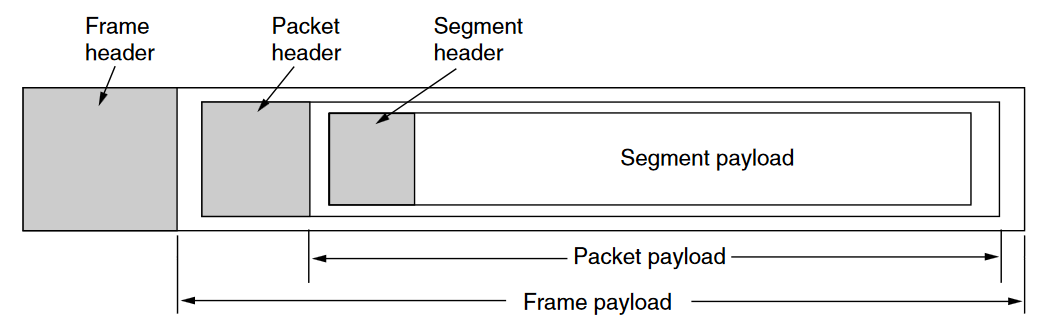
\includegraphics[width=14cm]{frames.png}
	\end{center}
	\caption{Nesting of segments, packets, and frames. \cite{tanenbaum}}
	\label{segments_packets_frames}
\end{figure}

\begin{figure}[ht]
	\begin{center}
		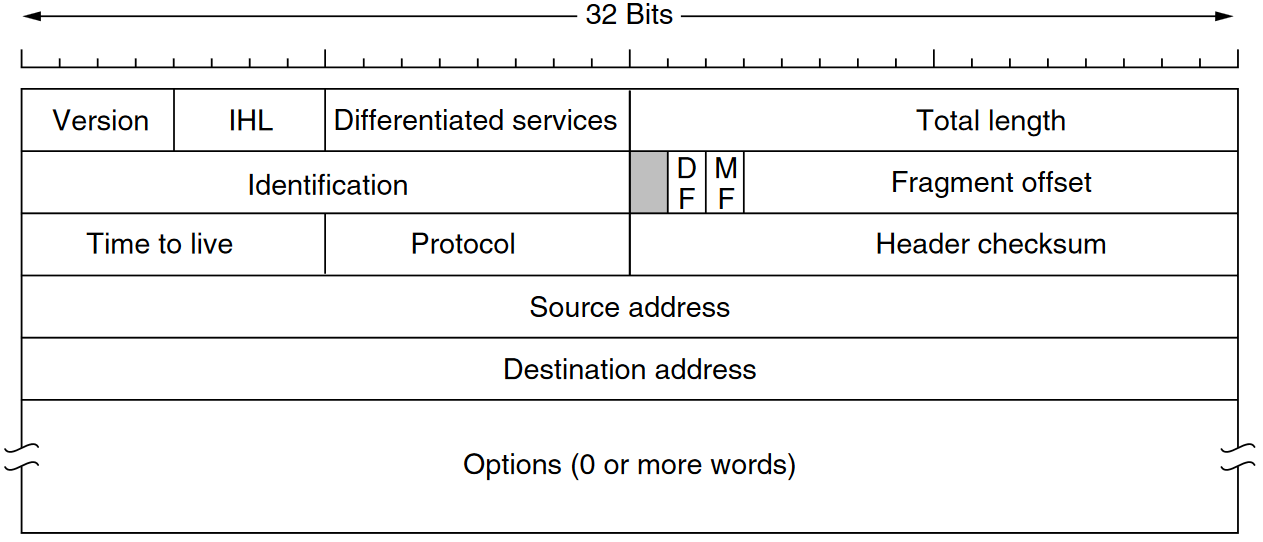
\includegraphics[width=14cm]{ip_header.png}
	\end{center}
	\caption{The IPv4 (Internet Protocol) header. \cite{tanenbaum}}
	\label{ip_header}
\end{figure}

\subsection{Software-Defined Networking}
\label{software_defined_networking}
% reference mininet and P4
% control plane vs data plane
  % what are these
  % Why is it good to separate them?
  % what are the drawbacks of separating them?



% from progress report
The primary benefit of SDN is that it gives the programmer more direct and clear control over how routing decisions are made. SDN aims to separate the network control, known as the control plane, from the forwarding proces, known as the data plane \cite{software_defined_networking_survey}. The control plane makes decisions about packets which are either destined to or originally from the current host, while the data plane makes decisions about packets which are going through the host. The control plane also maintains the routing table, which is used by both planes to make routing decisions.
